% !TeX root = ../main.tex
\cleardoublepage
\pagestyle{plain}
\refstepcounter{dummy}
\label{pap:paper6}
{\tikzexternaldisable 
    \begin{tikzpicture}[overlay,remember picture]
    \node[fill=black, rectangle, text width=4cm,
    text height=1.5em,anchor=north east, inner sep=12pt] 
    at ($ (current page.north east) + (-0cm,-3cm) $) 
    {\textcolor{white}{\HUGE Paper \uppercase\expandafter{\romannumeral6}}};
\end{tikzpicture}}
\vfill
\noindent
\LARGE \papersix
\vspace{0.5cm}

\normalsize\noindent
\authorsix

\vspace{2cm}

\cleardoublepage % the shim needs to appear on a righthandside page and the lefthandside page immediately following needs to be blank



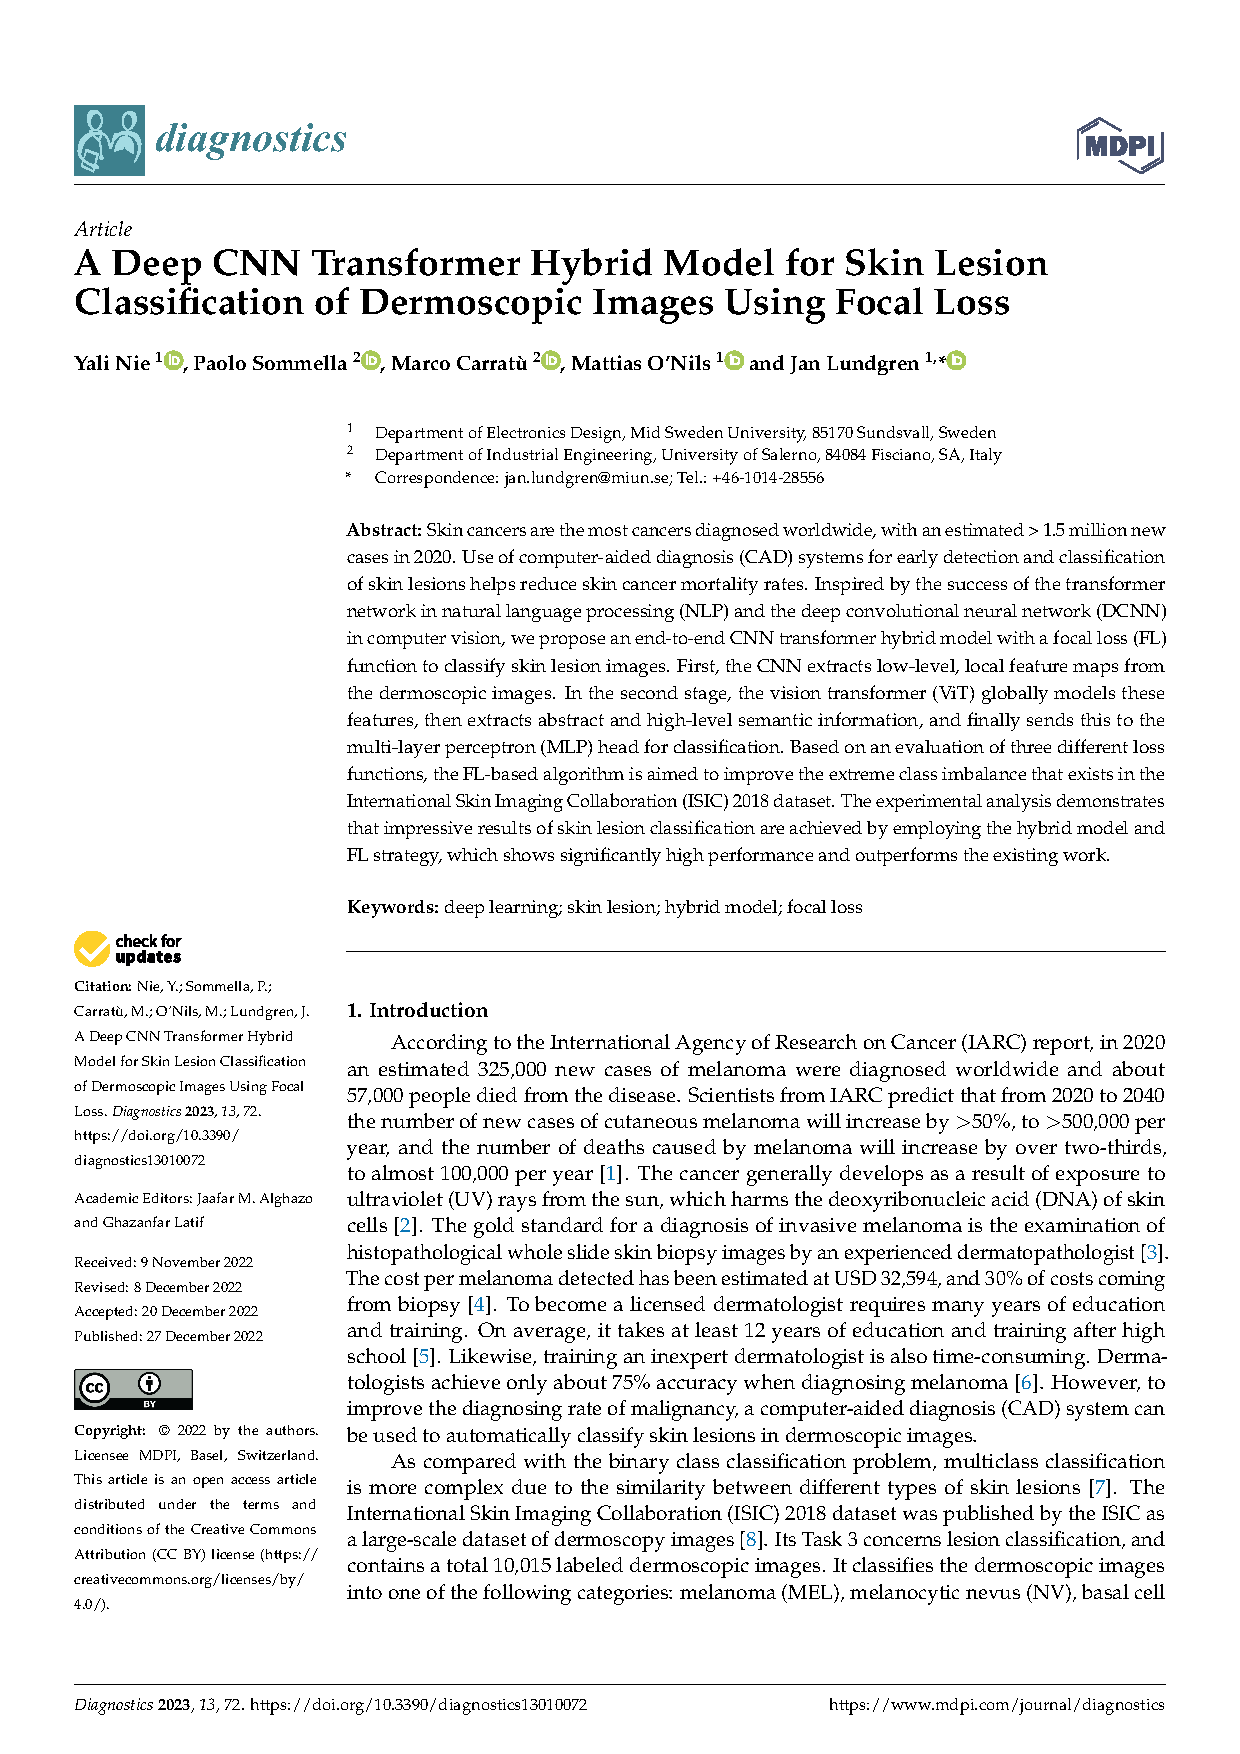
\includepdf[pages=1-,width=1.0\textwidth,pagecommand=\makeoddfoot{miunlic}{}{}{\small page | \thepage}, templatesize={169mm}{239mm}, frame=false, scale=1, trim=29mm 5mm 29mm 10mm, offset=-5 0]{papers/paper6.pdf} %note: I don't know why \makeoddfoot creates page numbers for both even and odd pages, but it seems to work
